\chapter{State of the art}
    \section{Windows Subsystem for Linux}
    Windows Subsystem for Linux (WSL) is a new and complex Windows component which implements a lot of new functionality (linux syscalls),
    parsing (ELF files parsing) and is based on existing Windows technologies, like pico providers and pico processes.
    
    This new optional feature was released in version 1607 of Windows 10 \cite{WindowsInternals}, also known as "Redstone 1" or
    "Anniversary Update".

        \subsection{Minimal Processes and Pico Processes}
            A minimal process has no process enviroment-block (PEB), no initial thread, ntdll is not loaded in its memory as it is done
            for all windows processes, and its address space is empty. However, a minimal process has a security token, a protection level,
            and a parent. Threads inside a minimal process are called "minimal threads". Similarly to minimal processes, minimal threads
            have no thread-enviroment block (TEB).

            A pico process is a minimal process, with an associated pico provider, which handles the system calls, exceptions, pico process
            or threads creation and termination.    

        \subsection{Pico Providers}
            A pico provider is a kernel driver that implements the required functionalities to handle the pico process events enumerated before.
            Essentially, a pico provider is a custom written kernel module that implements the necessary callbacks to respond to the list of
            possible events (shown earlier) that a Pico process can cause to arise\cite{WindowsInternals}. Drivers can register as pico providers by calling the
            PsRegisterPicoProvider API, however, calling this API requires that the PspPicoRegistrationDisabledis set to FALSE. This value is
            set to false before any other third party driver is loaded.
            
            Securing pico providers is done with the help of PatchGuard in order to protect its syscalls handlers. Kernel Patch Protection,
            also known as PatchGuard, was designed to protect kernel structures from being patched. This renders the classic linux
            monitoring solution (syscall hooking) useless, as any attempt to hook the syscalls will result in a Blue Screen of Death (BSOD).


        Linux processes are implemented as pico processes which have lxcore as their associated pico provider, thus the reason why lxcore
        implements the Linux syscalls.


        \subsection{WSL Components}
            The main components of WSL are:
            \begin{itemize}
                \item lxcore.sys
                \item lxss.sys
                \item LxssManager
                \item init
            \end{itemize}

            \begin{figure}[H]
                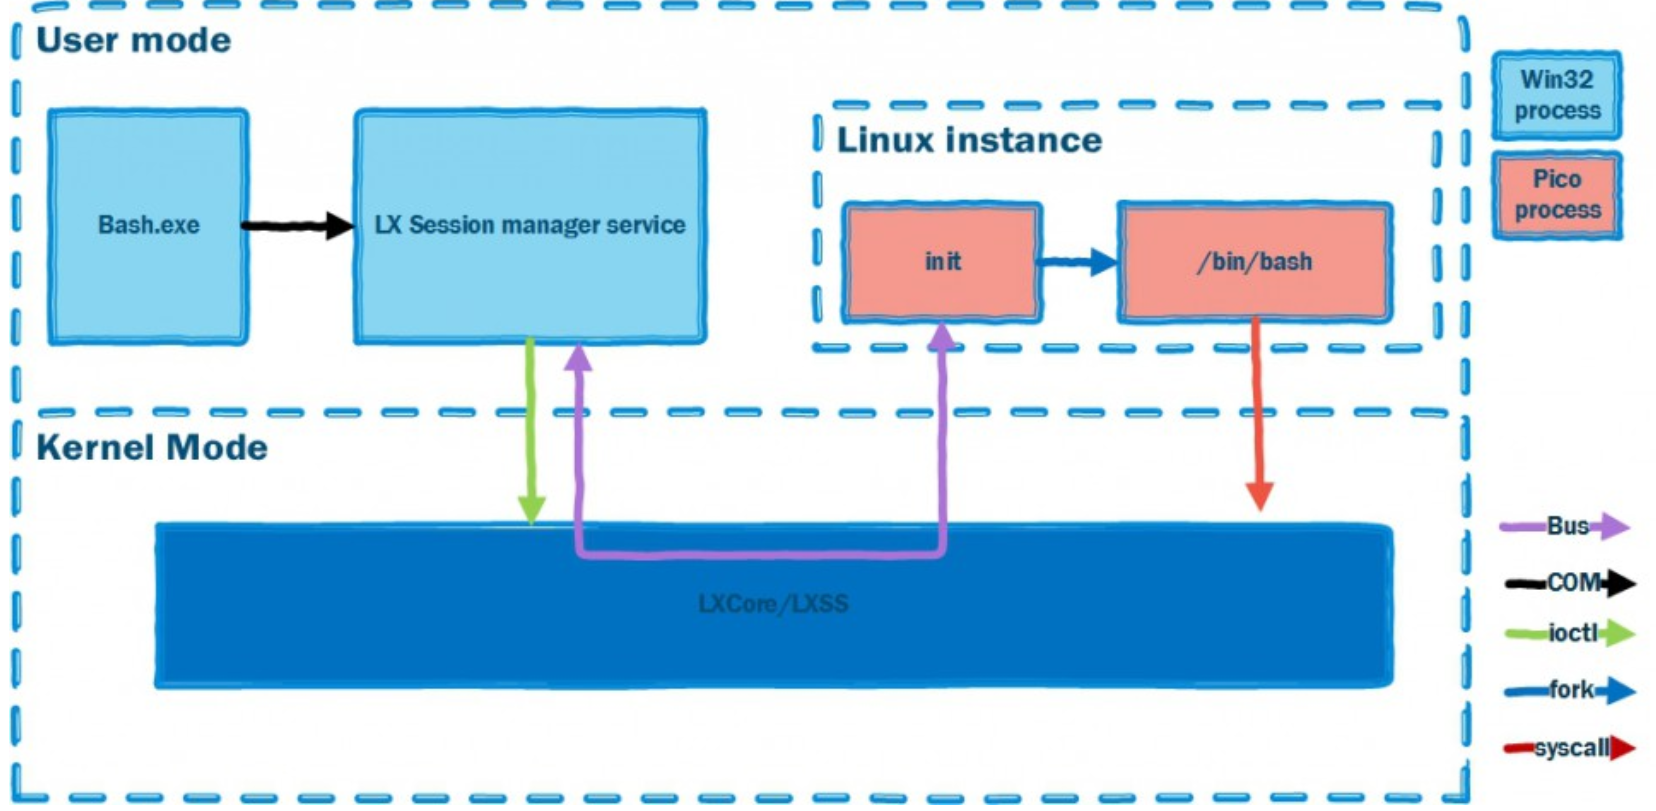
\includegraphics[width=\linewidth]{img/wsl_components.png}
                \caption{WSL Compoents}
                \label{fig:wsl_components}
            \end{figure}

            \subsubsection{Lxss.sys}
            Lxss.sys is reponsible for initialing the WSL enviroment by calling the LxInitialize function exported by lxcore.sys, as it can be
            seen below.

            \begin{figure}[H]
                \centering
                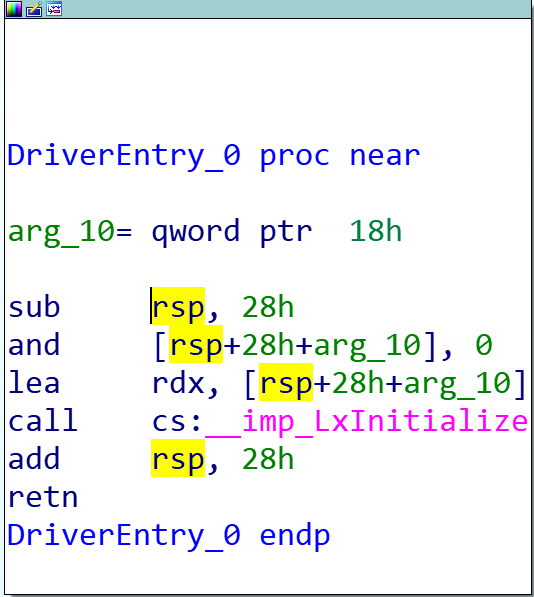
\includegraphics[width=150px, keepaspectratio]{img/lxss.png}
                \caption{Lxss.sys}
                \label{fig:lxss}
            \end{figure}

            This being its only responsability, it is currently not of great interest.
            
            \subsubsection{Lxcore.sys}
            Lxcore is the pico provider driver which implements the Linux-compatible kenel API and ABI, as well as a device object for command
            and control\cite{Bluehat2016AI}, making it the core component of WSL. Over 200 syscalls are implemented in lxcore as well as
            multiple file systems.

            \paragraph{}
            Exposes the ADSS communication bus in order to enable communication between Windows applications and linux applications. Windows
            applications need to register a server on the ADSS using the ILxssSesion COM interface. The linux application has to open the
            "/dev/lxss" and connect to the server by sending the correct ioctl. This is currently undocumented and undocumented
            method of communicating between linux and windows processes and is prone to changes.

            \subsubsection{LxssManager}
            LxssManager is a user-mode service which provides a COM interface and communicates with lxcore through its Device Object
            (\textbackslash Device\textbackslash Lxss). Is is responsible with starting the init process of a WSL instance and, as shown
            in \ref{fig:wsl_components}, does so with the help of lxcore through the ADSS bus.

            \subsubsection{init}
            The init daemon process is the well known linux root process (first process started by the kernel), making it the ancestor for
            every other Linux process. A new init daemon process is created for each WSL instance.


        \subsection{WSL File Systems}
            Lxcore implements multiple file systems in order to cover well known linux functionality as well as WSL and Windows interoperability.


            \begin{itemize}
                \item VFS (virtual file system)
                \item DrvFs for Linux files system that maps Windows drives, LxFs, 
                \item VolFs for the linux file system
                \item ProcFs for /proc
                \item SysFs for /sys
                \item TmpFs for /tmp
            \end{itemize}

            VFS provides an interface indepentent of the underlying file system. In this model, all file system operations go through the
            same interface, regardless of the underlying file system type\cite{TheArtOfMemoryForensics}.

            \begin{figure}[H]
                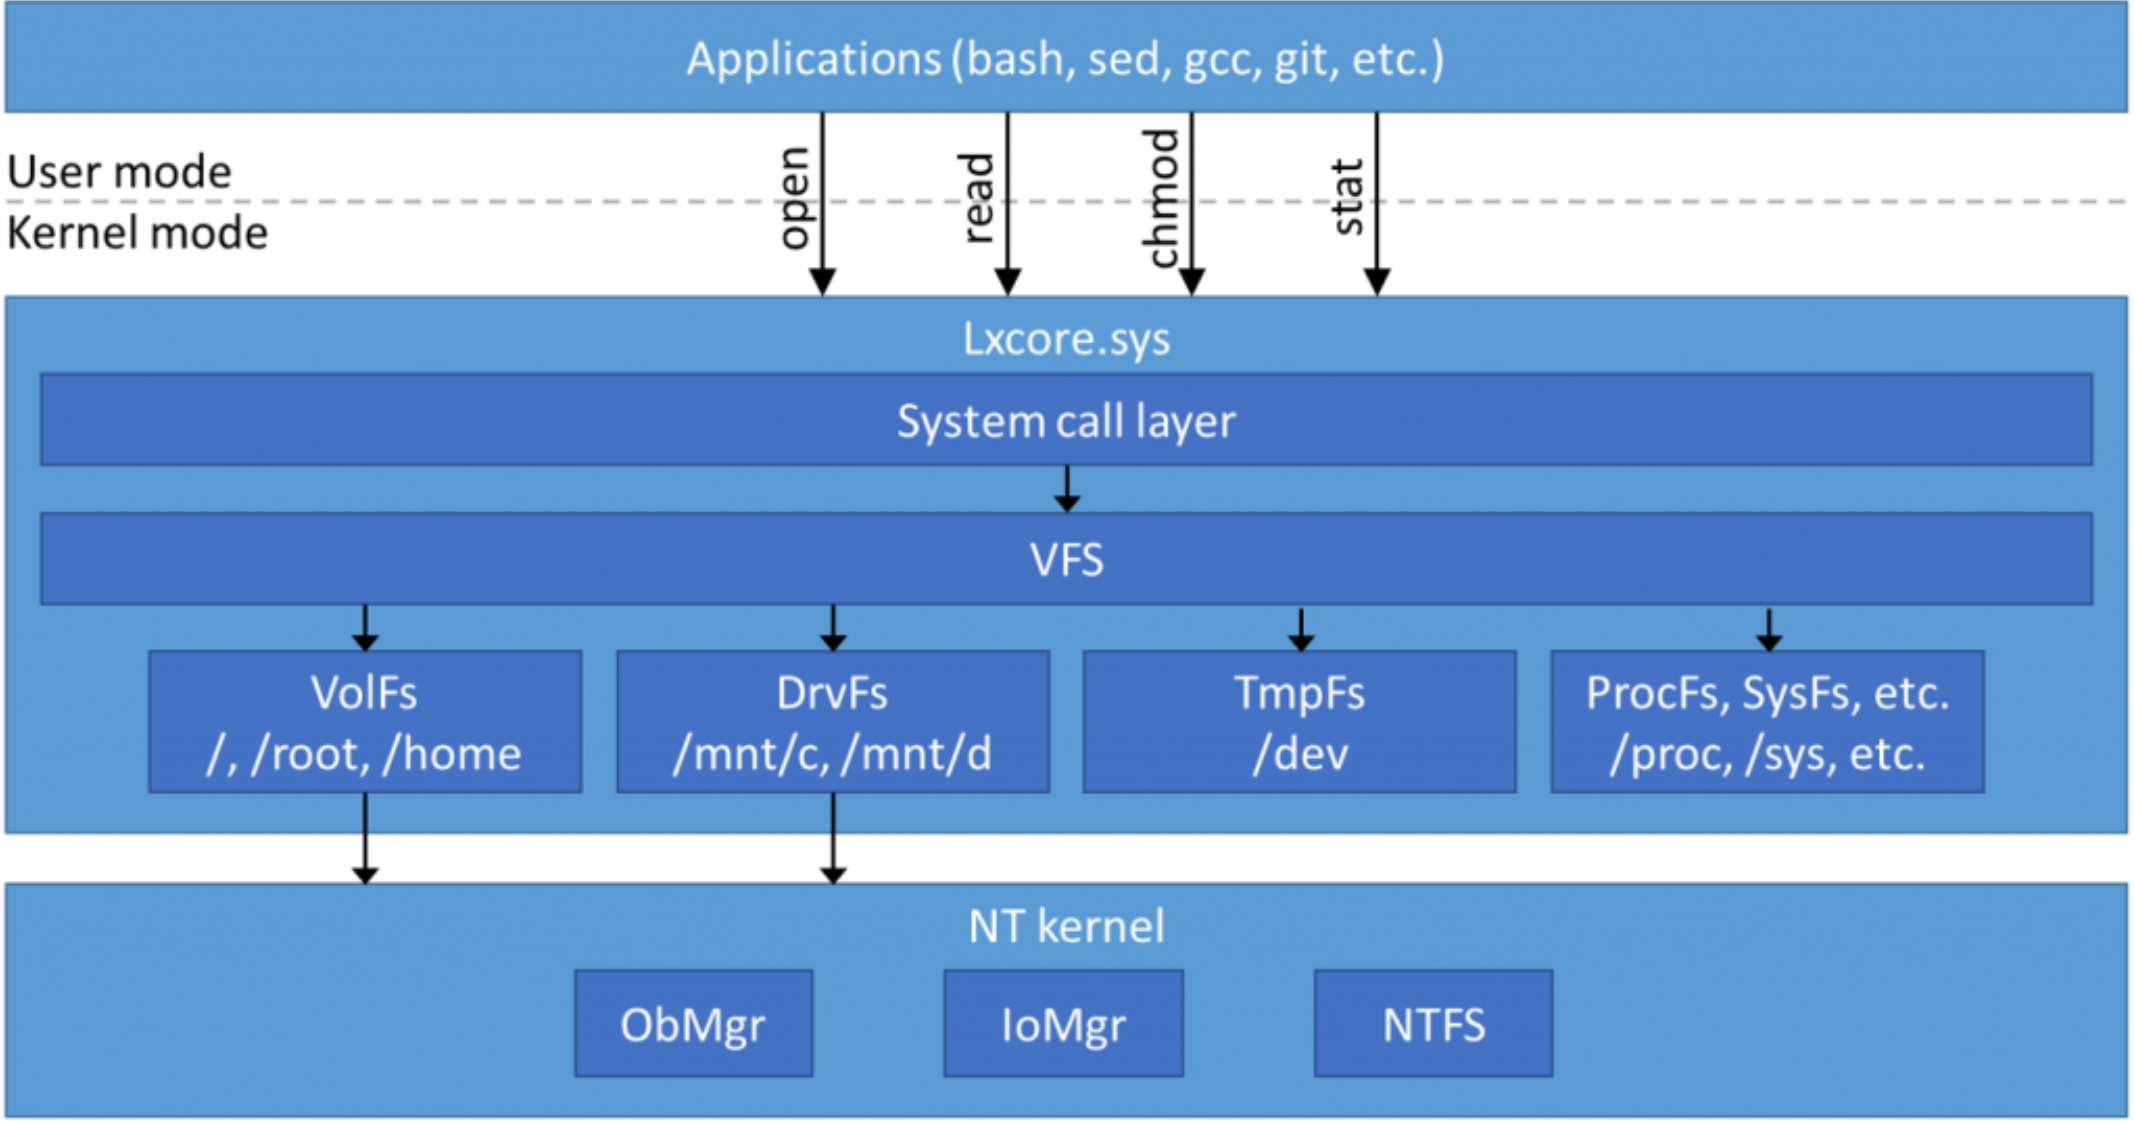
\includegraphics[width=\linewidth]{img/wsl_file_system.png}
                \caption{WSL File System}
                \label{fig:wsl_file_system}
            \end{figure}

            As can be seen in \ref{fig:wsl_file_system}, VolFs and and DrvFs operations actually redirected to the Windows kernel after some
            pre processing, while the requests for the other file systems are resolved by lxcore.
        
        \subsection{Security Issues}
            When WSL was first released, multiple monitorinig and analysis tools encountered issues in identifying and displaying information
            about Linux processes. For example, as it can be seen in the following picture, procmon had issues displaying the commandline a process
            was started with:

            \begin{figure}[!htp]
                \centering
                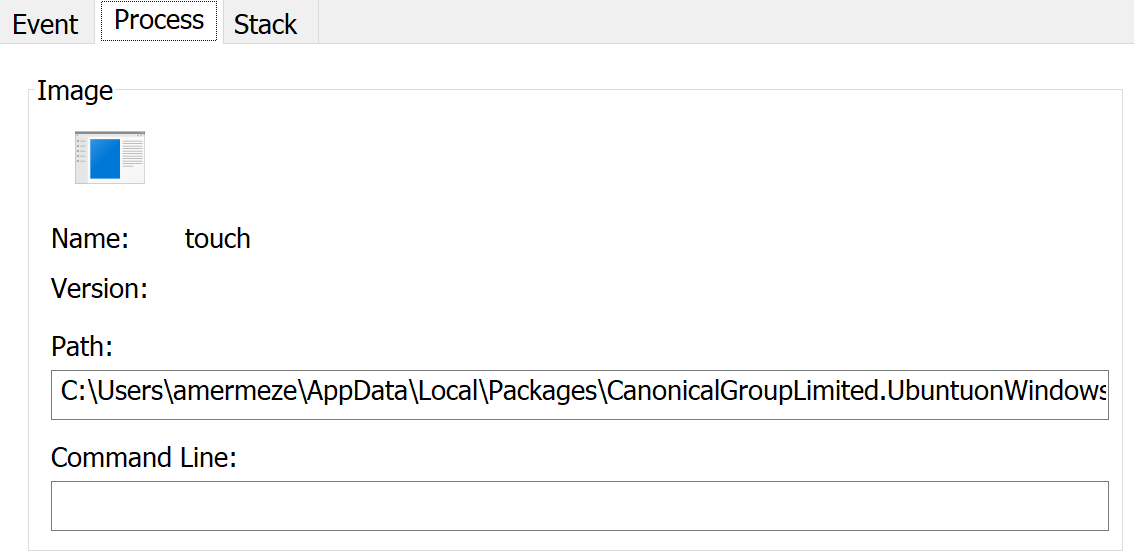
\includegraphics[width=300px, keepaspectratio]{img/procmon.png}
                \caption{commandline for "touch file"}
                \label{fig:procmon}
            \end{figure}

            \paragraph{}
            Callbacks registered for process notifications with the old APIs (PsSetCreateProcessNotifyRoutine and
            PsSetCreateProcessNotifyRoutineEx) were not called for pico processes, therefore activity monitors would not know of Linux processes.
            In order to receive notification for pico processes too, a new API called PsSetCreateProcessNotifyRoutineEx2 had to be used, meaning
            that all activity monitor drivers had to be updated to use the new API if available.

            Moreover, since most activity monitors would not filter I/O activity done by the kernel, Linux process I/O activity would not be
            filtered, because lxcore issues IRPs on behalf of the process that started the I/O operation.

    \section{Malware, Bashware and Exploits}
        Software that “deliberately fulfills the harmful intent of an attacker” is commonly referred to as malicious software or malware
        \cite{ieeeproc2007}.

        Bashware is a type of malware that leverages WSL in order to bypass monitoring tools and anti-virus products in order to do damage to the
        operating system.
        
        \subsection{execve exploit}
            Discovered in February 2018 by Saar Amar, security researcher, execve exploit\cite{execve} is a privilege escalation exploit that
            leverages a vulnerability in lxcore, more exactly an integer overflow in LxpUtilReadUserStringSet. Starting from this vulnerability,
            the exploit proof of concept copies the system security token over another process' security token, elevating it at runtime.

        \subsection{File Infector}
            A WSL file infector would essentially inject into windows executable files, altering the code in order to deliver some malicious
            code. Even though this can generally be prevented by software developers by signing their binaries, assuring that, if loaded, were
            not tampered with, unsigned binaries still exist and are vulnerable to being hijacked.
            
        \subsection{Local Denial of Service}
            A local denial of service exploit would greatly distrupt the user experience by causing considerable slow-down of 
            the machine, crashes, freezes, essentially preventing the user from using the machine.

            \paragraph{}
            While experimenting with Event Tracing for Windows (ETW) I've found a way of consistently causeing lxcore.sys to run into a BSOD, 
            due to an access violation exception. This can be triggerd from a normal process with no admin rights. I will not go into more 
            detail about this yet, as it would not respect the responsible disclosure policy, since it wasn't yet fixed by Microsoft. Releasing
            information about how to trigger this local denial of service attack could cause exploitation in the wild.

    \pagebreak
    
    \section{Behavioral Detection}
        One traditional way of detecting malware is matching the executable file against a set of static, pre generated, signatures. These
        signatures are created in a way so that they only match malicious software\cite{ASADMATT}. The problem with signature-based detection
        is that signature extraction is time consuming, and, once extracted, the anti-virus product must be updated with the new signatures.
        Moreover, the signature could be rendered useless if the parts from the malware that were used in the signature are modified, if
        the malware code is encrypted or if the malware modifies its code at runtime. This leaves the user vulnerable to new "0-day" threats. 

        \paragraph{}
        As stated in \citetitle{jacob2008behavioral}, a behavioral detector needs to monitor the actions of a program and identify actions
        which betray a malicious intent or activity. In the past, interrupt filtering was the main method of gathering information about a
        program's behavior. Later it was replaced by hooking system calls (Linux or older Windows version). The modern approach of intercepting
        a program's actions on Windows systems is to use technologies and APIs that reside in the operating system. For example, using a
        minifilter driver for intercepting file system activity, or using the PsSetCreateProcessNotifyRoutine API to intercept process
        creation and termination.

        \paragraph{}
        Unlike signature based anti-malware solutions, which is used to detect already known malware, behavioral detection has the advantage of
        detecting 0-day threats. A behavioral detection anti-malware solution would analyze and evaluate a running process' actions in order to
        determine whether it is malicious or not. There are many examples of potentially malicious behavior, ranging from assuring persistence on
        the system to injecting and hijacking other processes.

        One obvious disadvantage is the performance overhead that comes with analyzing the behavior of a running process. Another disadvantage is
        that the process might be able to cause some damage before being stopped by the anti-malware solution, as an example, a ransomware might
        encrypt a few files or fragments of files before it is stopped.
        